\subsubsection{DSU - Disjoint Set Union (Union-Find)}
A estrutura de dados Disjoint Set Union (DSU) é utilizada para rastrear um
conjunto de elementos particionados em vários subconjuntos disjuntos (não
sobrepostos). Ela suporta duas operações principais quase em tempo constante,
$\mathcal{O}(\alpha(V))$, graças às otimizações de \textbf{compressão de
    caminho} e \textbf{união por tamanho}: a operação \textit{Find} (descobre a
qual conjunto um elemento pertence) e a \textit{Union} (une dois conjuntos).

\paragraph{Pseudo-Código: }\mbox{}\\
\begin{algorithm}[H]
    \SetAlgoLined
    \SetKwFunction{Find}{Find}
    \SetKwFunction{Union}{Union}
    \SetKwProg{Fn}{Função}{:}{}

    \Fn{\Find{$x$}}{
        \Se{$pai[x] == x$}{
            \Retorna $x$\;
        }
        $pai[x] \gets$ \Find{$pai[x]$} \text{ // Compressão de caminho}\;
        \Retorna $pai[x]$\;
    }

    \vspace{0.2cm}

    \Fn{\Union{$x, y$}}{
        $raizX \gets$ \Find{$x$}\;
        $raizY \gets$ \Find{$y$}\;

        \Se{$raizX \neq raizY$}{
            \text{// União por tamanho (liga o menor ao maior)}\;
            \Se{$tamanho[raizX] < tamanho[raizY]$}{
                \text{Trocar os valores de } $raizX$ \text{ e } $raizY$\;
            }
            $pai[raizY] \gets raizX$\;
            $tamanho[raizX] \gets tamanho[raizX] + tamanho[raizY]$\;
        }
    }
    \caption{Disjoint Set Union (DSU)}
\end{algorithm}

Veja a estrutura do DSU sendo formada (as setas apontam para o pai):\\
\vspace{0.5cm} \noindent
\begin{minipage}[t]{0.31\textwidth}
    \centering
    \textbf{Passo 1: Inicialização}\\
    \vspace{0.2cm}
    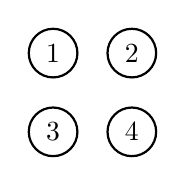
\begin{tikzpicture}[every node/.style={circle, draw, minimum size=0.5cm, thick}]
        \node (1) at (0, 0) {1};
        \node (2) at (1, 0) {2};
        \node (3) at (0, -1) {3};
        \node (4) at (1, -1) {4};
    \end{tikzpicture}

    \vspace{0.2cm}
    \footnotesize
    \raggedright
    Cada elemento é seu próprio pai. Nenhum conjunto foi unido ainda.
\end{minipage}%
\hfill
%
\begin{minipage}[t]{0.31\textwidth}
    \centering
    \textbf{Passo 2: Union(1, 2) e Union(3, 4)}\\
    \vspace{0.2cm}
    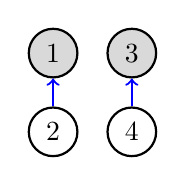
\begin{tikzpicture}[every node/.style={circle, draw, minimum size=0.5cm, thick}]
        \node[fill=gray!30] (1) at (0, 0) {1};
        \node (2) at (0, -1) {2};
        \node[fill=gray!30] (3) at (1, 0) {3};
        \node (4) at (1, -1) {4};
        \draw[->, thick, blue] (2) -- (1);
        \draw[->, thick, blue] (4) -- (3);
    \end{tikzpicture}

    \vspace{0.2cm}
    \footnotesize
    \raggedright
    1 e 3 tornam-se raízes dos seus respectivos conjuntos.
\end{minipage}%
\hfill
%
\begin{minipage}[t]{0.31\textwidth}
    \centering
    \textbf{Passo 3: Union(1, 3)}\\
    \vspace{0.2cm}
    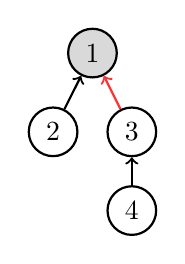
\begin{tikzpicture}[every node/.style={circle, draw, minimum size=0.5cm, thick}]
        \node[fill=gray!30] (1) at (0.5, 0) {1};
        \node (2) at (0, -1) {2};
        \node (3) at (1, -1) {3};
        \node (4) at (1, -2) {4};
        \draw[->, thick] (2) -- (1);
        \draw[->, thick, red!80] (3) -- (1);
        \draw[->, thick] (4) -- (3);
    \end{tikzpicture}

    \vspace{0.2cm}
    \footnotesize
    \raggedright
    Ambos tinham tamanho 2. O nó 1 se torna o pai do nó 3. Todos agora no mesmo conjunto.
\end{minipage}

\paragraph{Implementação: }\mbox{}
\textbf{Python: }
\begin{lstlisting}[language=Python]
class DSU:
    def __init__(self, n):
        self.pai = list(range(n))
        self.tamanho = [1] * n
        
    def find(self, x):
        if self.pai[x] == x:
            return x
        # Compressao de caminho
        self.pai[x] = self.find(self.pai[x])
        return self.pai[x]
        
    def union(self, x, y):
        raiz_x = self.find(x)
        raiz_y = self.find(y)
        
        if raiz_x != raiz_y:
            # Uniao por tamanho
            if self.tamanho[raiz_x] < self.tamanho[raiz_y]:
                raiz_x, raiz_y = raiz_y, raiz_x
                
            self.pai[raiz_y] = raiz_x
            self.tamanho[raiz_x] += self.tamanho[raiz_y]
            return True # Ocorreu uniao
        return False # Ja estavam no mesmo conjunto
\end{lstlisting}

\vspace{0.3cm}
\textbf{C++:}
\begin{lstlisting}[language=C++]
struct DSU {
    vector<int> pai, tamanho;
    
    DSU(int n) {
        pai.resize(n);
        tamanho.assign(n, 1);
        iota(pai.begin(), pai.end(), 0); // Preenche 0, 1, ..., n-1
    }
    
    int find(int x) {
        if (pai[x] == x) return x;
        return pai[x] = find(pai[x]); // Compressao de caminho
    }
    
    bool unite(int x, int y) {
        int raizX = find(x);
        int raizY = find(y);
        
        if (raizX != raizY) {
            // Uniao por tamanho
            if (tamanho[raizX] < tamanho[raizY]) swap(raizX, raizY);
            pai[raizY] = raizX;
            tamanho[raizX] += tamanho[raizY];
            return true;
        }
        return false;
    }
};
\end{lstlisting}
\newpage